\begin{figure}[b]
%% \begin{figure}[h]
  \centering
  \begin{tikzpicture}[nodes = {align = left}]
    %% \node [scale=.45]
    \node [scale=.33]
    {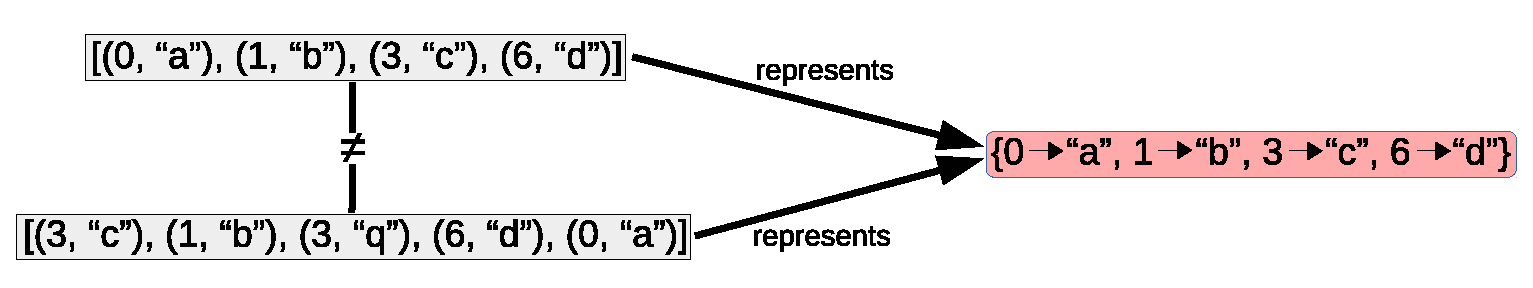
\includegraphics{figs/unequal.eps}};
  \end{tikzpicture}
  \caption{Two distinct \sal{}s representing the same semantic mapping. \rkc{Let's show the first two rows from Fig 1. And let's fit this into one column.} \rkc{Actually, maybe the semantic mapping should just be shown inside Fig 1.}}
  \label{fig:uneq}
\end{figure}
